\documentclass{standalone}
\usepackage{tikz}
\usetikzlibrary{decorations.pathmorphing}
\usepackage{pgfplots}
\pgfplotsset{compat=1.11}
\usepgfplotslibrary{fillbetween}
\usetikzlibrary{intersections}
\begin{document}
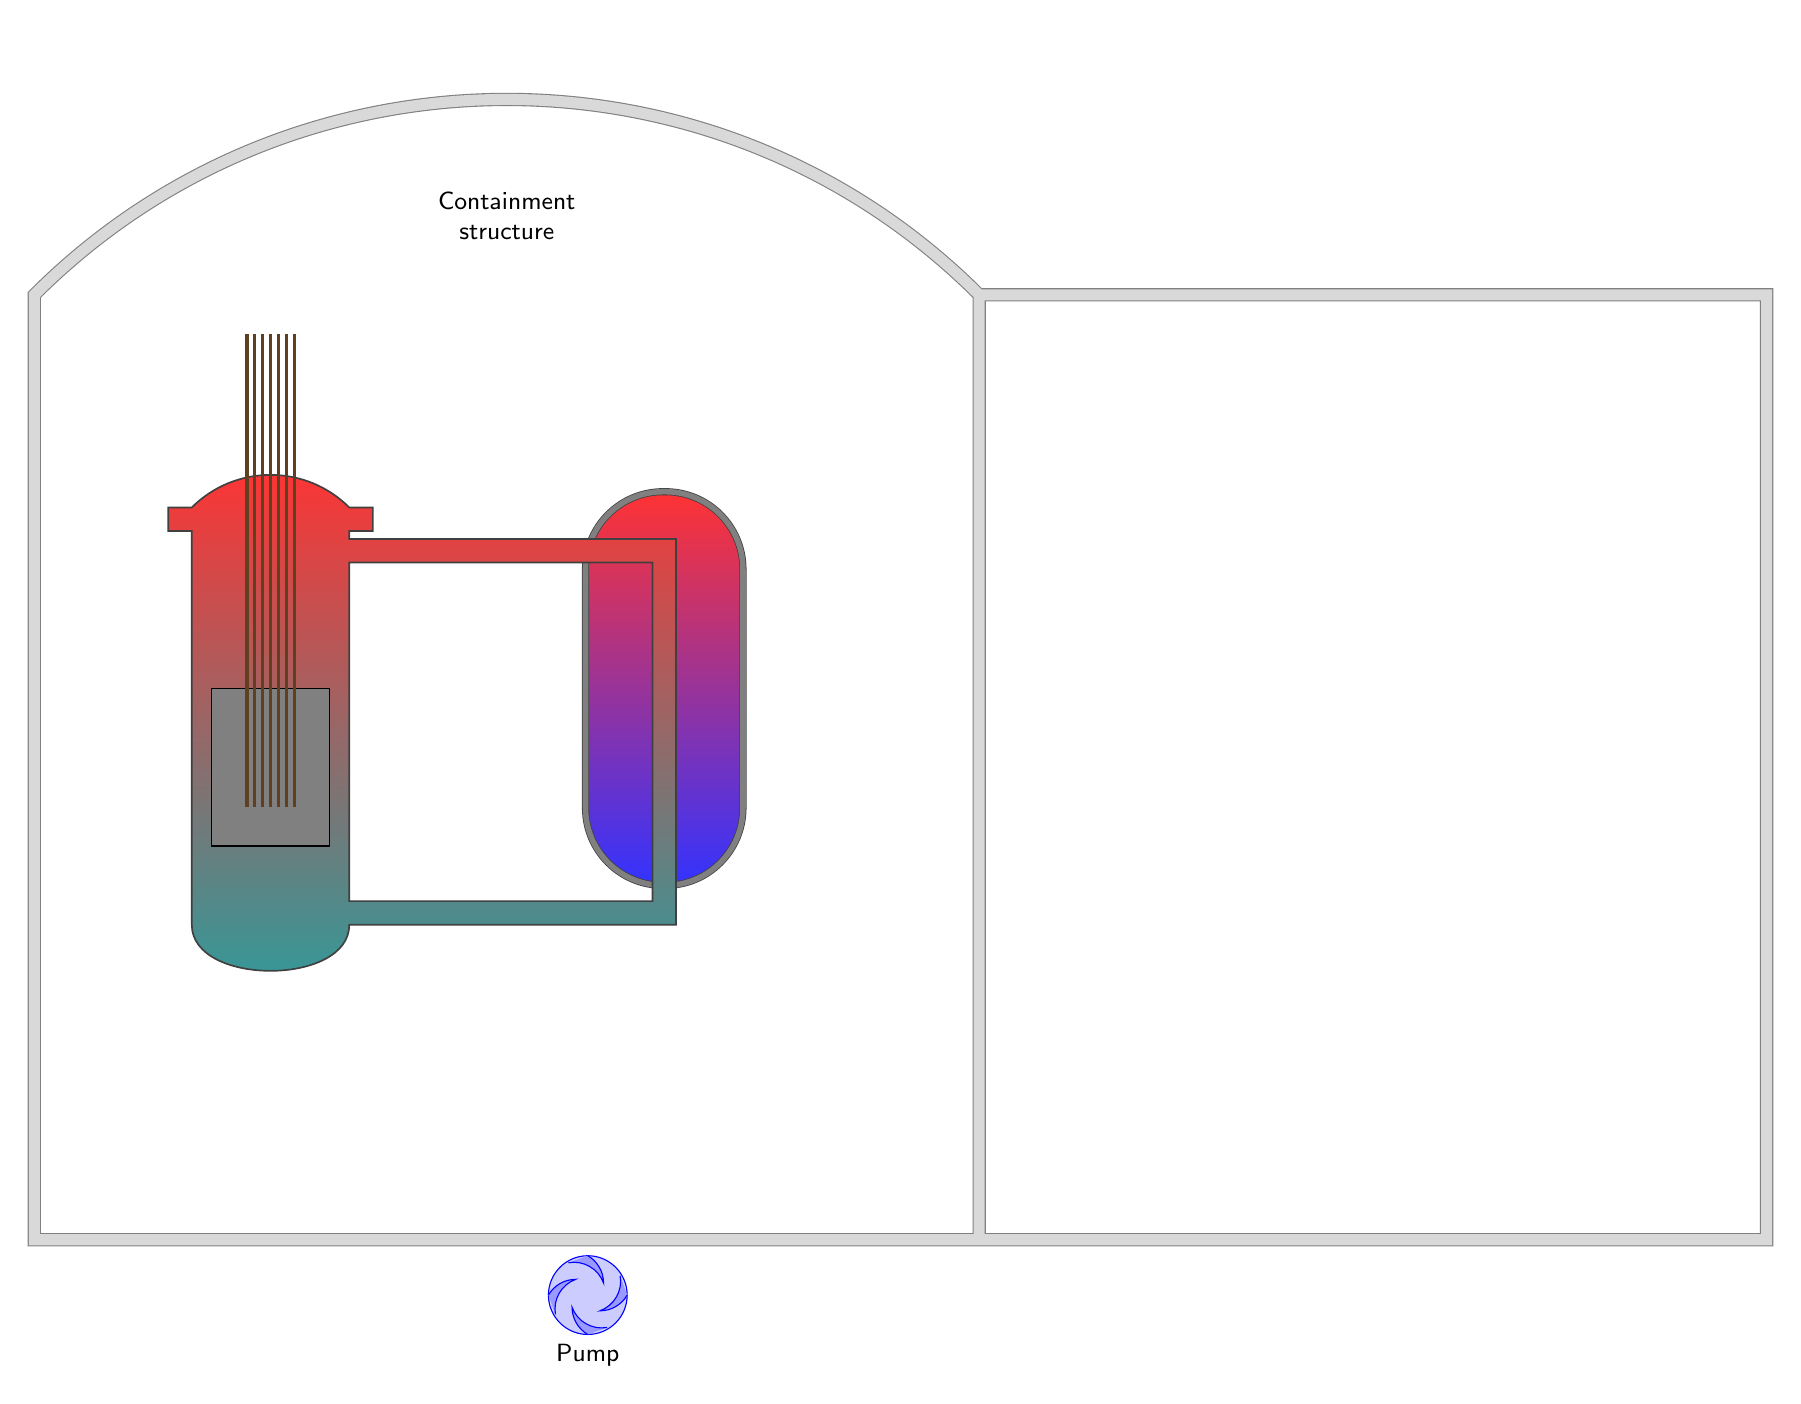
\begin{tikzpicture}
  \sffamily
  \draw[draw=gray,double=gray!30,double distance=4pt]
  (12,12) to[out=135,in=45](0,12)--(0,0)--(22,0)--(22,12)--(12,12)--(12,0);
  \node[text width=4cm, text centered,font=\small] at (6,13)
  {Containment\\structure};

  \begin{scope}[xshift=200,yshift=-20]
    \filldraw[fill=blue!20,draw=blue] (0,0) circle (0.5cm);
    \node[below,font=\small] at (0,-0.5) {Pump};
    \filldraw[fill=blue!40,draw=blue,yshift=-0.5cm]
    (0,0) arc (240:180:0.4cm)  arc (200:280:0.4cm) ;
    \filldraw[fill=blue!40,draw=blue,yshift=+0.5cm,rotate=180]
    (0,0) arc (240:180:0.4cm)  arc (200:280:0.4cm) ;
    \filldraw[fill=blue!40,draw=blue,xshift=+0.5cm,rotate=90]
    (0,0) arc (240:180:0.4cm)  arc (200:280:0.4cm) ;
    \filldraw[fill=blue!40,draw=blue,xshift=-0.5cm,rotate=-90]
    (0,0) arc (240:180:0.4cm)  arc (200:280:0.4cm) ;
  \end{scope}

  \node[rectangle,draw=darkgray,double=gray,line width=0.1mm,minimum width = 2cm,minimum height = 5cm,rounded corners=28pt,double distance=2pt,top color = red!80,bottom color=blue!80] at (8,7){};

  \filldraw[semithick,draw=darkgray,top color=red!80,bottom color=teal!80]
  % outer outline (clockwise)
  (2,9)--(2,4) to[out=270,in=270](4,4)--(8+0.15,4)--(8+0.15,8.9)--(4,8.9)--(4,9)--(4.3,9)--(4.3,9.3)--(4,9.3) to[out=135,in=45](2,9.3)--(1.7,9.3)--(1.7,9)--cycle
  % inner outline (counter-clockwise)
  (4,4+0.3)--(4,8.9-0.3)--(8-0.15,8.9-0.3)--(8-0.15,4+0.3)--cycle;

  % core
  \node[rectangle,draw=black,fill=gray,minimum width = 1.5cm,minimum height = 2cm] at (3,6){};

  % control roads
  \foreach \i in {1,...,7}{
      \draw[very thick,brown!50!black] (2.6+\i*0.1,5.5)--(2.6+\i*0.1,11.5);
    }
\end{tikzpicture}
\end{document}
